\documentclass{beamer}
\usepackage{amsmath}
\usepackage{listings}
\usepackage{xcolor}
\usepackage{multirow}
\usepackage{amssymb}
\usepackage{setspace}
\usepackage{amsmath}
\usepackage{listings}
\usepackage{xcolor}
\usepackage{multirow}
\usepackage{amssymb}
\usepackage{pgfplots}
\usepackage{pgfplotstable}
\usepackage{float}
\AtBeginDocument{%
      \DeclareSymbolFont{pureletters}{T1}{lmr}{\mddefault}{it}%
      }

\usepgfplotslibrary{fillbetween}
\usetikzlibrary{arrows.meta, bending}
\pgfplotsset{compat=newest}
\usetikzlibrary{decorations.markings}
\usepackage{pgfplotstable}
\usepackage{float}
\usepackage{tikz}

\usepackage{pgfplots}
\usepgfplotslibrary{dateplot}
\usetheme{Madrid}
\usecolortheme{default}

\title[Financial Frictions \& Cleansing Effects]{Financial Frictions and the Cleansing Effects of Recessions}
\author[Riccardo Dal Cero]{Dissertation by: Riccardo Dal Cero \\{\small Supervisor: Domenico Delli Gatti} }
\date[09/04/24]{ A.Y. 2022/2023}
\logo{
\includegraphics[scale=0.2]{logo.png}}
\institute{Università Cattolica del Sacro Cuore \\ Campus of Milan}
\setbeamertemplate{footline}{
  \leavevmode%
  \hbox{%
  \begin{beamercolorbox}[wd=.4\paperwidth,ht=2.25ex,dp=1ex,center]{author in head/foot}%
    \usebeamerfont{author in head/foot}\insertshortauthor
  \end{beamercolorbox}%
  \begin{beamercolorbox}[wd=.3\paperwidth,ht=2.25ex,dp=1ex,center]{title in head/foot}%
    \usebeamerfont{title in head/foot}\insertshorttitle
  \end{beamercolorbox}%
  \begin{beamercolorbox}[wd=.3\paperwidth,ht=2.25ex,dp=1ex,right]{date in head/foot}%
    \usebeamerfont{date in head/foot}\insertshortdate{}\hspace*{2em}
    \insertframenumber{} / \inserttotalframenumber\hspace*{2ex} 
  \end{beamercolorbox}}%
  \vskip0pt%
}
\AtBeginSection[]
{
  \begin{frame}
    \frametitle{Table of Contents}
    \tableofcontents[currentsection]
  \end{frame}
}
\begin{document}
\frame{\titlepage}

\begin{frame}
    \frametitle{Motivations}
    \begin{itemize}
        \item Economic downturns are associated with increased patterns of reallocation.
        \item Literature on the Cleansing Effect suggests that these patterns are a productivity-enhancing phenomenon (Caballero \&
        Hammour, 1993)
        \item This pattern shifted during the Great Recession (as identified by Foster, Grim, \& Haltiwanger,
        2016): the intensity of reallocation 
        fell rather than rise
    \end{itemize}
\end{frame}


\begin{frame}
    \frametitle{Research Questions}
    \begin{enumerate}
        \item How do \textbf{financial frictions} influence firms' decisions on optimal \textit{capital} and \textit{dividend} paths?
        \begin{itemize}
            \item By developing a \textbf{theoretical model} incorporating financial frictions
        \end{itemize}
        \item What are the \textit{aggregate-level} effects of financial frictions on the \textbf{cleansing effect}?
        \begin{itemize}
            \item Employing Monte Carlo simulations to investigate the impact of financial frictions
        \end{itemize}
    \end{enumerate}
\end{frame}
\section{The firm's problem}
\begin{frame}
    \frametitle{Flow of fund constraints and financial frictions}
The flow of funds constraint is:

    \begin{equation}
        k_{t+1}=k_{t}(1-\delta)- R b_{t} - d_t + f{(k_{t})}+b_{t+1} \label{c1}
    \end{equation}

Two types of financial frictions are included:
\begin{enumerate}
    \item \textbf{Monitoring costs} of the financial intermediaries (\(1-\mu\)) on the participation constraint:

            \begin{equation}
                R_t=\frac{R_f}{p}  -\frac{ 1-p }{ p }\frac{\mu f{(k_{t})}}{b_t} \label{c2}
            \end{equation}

    \item \textbf{Financing constraint}:

        \begin{equation}
            b_t = l \cdot k_t  \label{c3}
        \end{equation}
 
\end{enumerate}

\end{frame}

\begin{frame}{The firm's inter-temporal problem}
     The firm's objective is to maximize:

\[
\max_{{\{d_{t}\}}_{t=0}^{+\infty}}V_0 = \sum_{t=0}^{+\infty}{\beta^t U(d_t)}
\]

subject to: (\ref{c1}),(\ref{c2}),(\ref{c3}).
From the FOCs, we get:
\begin{block}{Euler equations for dividends}
    \begin{equation}
        U^{\prime}{(d_{t})}=\frac{\beta}{\left(1-l\right)} U^{\prime}{(d_{t+1})}\left[ f^{\prime}{(k_{t})}\frac{p + \mu - \mu p}{p} + \frac{p - \delta p - R_f l}{p} \right]
    \end{equation}
\end{block}
\end{frame}
\begin{frame}{Phase Diagram}
\begin{figure}
    \centering
    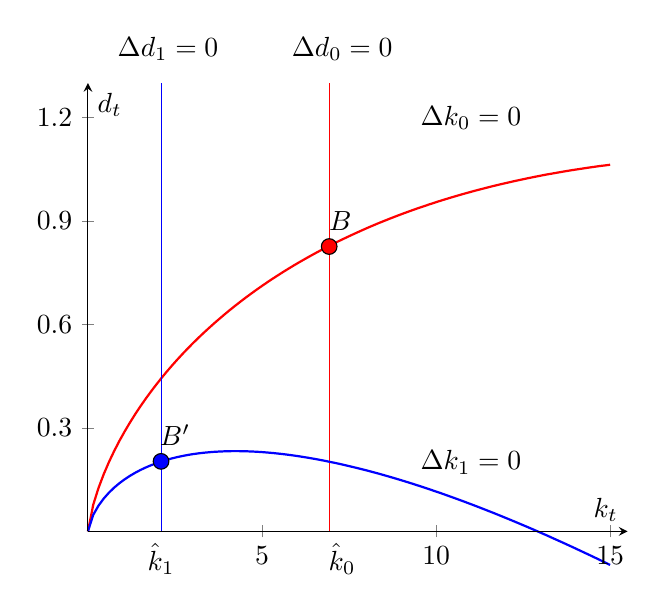
\begin{tikzpicture}
        \begin{axis}[
            axis lines=middle, % sets the position of the axes
            xlabel=\(k_t\),
            ylabel=\(d_t\),
            xmin=0, ymin=0,
            xmax=15.5, ymax=1.3,
            % Removed ticks=none to enable ticks
            clip=false,
            axis on top=true,
            xtick={0,5,...,20}, % Adds ticks at intervals of 5 on the x-axis
            ytick={0,0.3,...,1.3}, % Adds ticks at intervals of 0.3 on the y-axis
            xticklabel style={/pgf/number format/fixed},
            yticklabel style={/pgf/number format/fixed}
        ]
        
        % Parabolic curve without monitoring costs
        \addplot [
            color=red,
            domain=0:15, 
            samples=100, 
            thick,
        ]
        {0.5*x^0.8-0.22*x};
        \node at (axis cs:11,1.2) {\(\Delta{k_0}=0\)};
        %optimal capital without monitoring costs
        \draw [color=red] (axis cs:6.9296,0) -- (axis cs:6.9296,1.3);
        \node at (axis cs:7.3,1.4) {\(\Delta{d_0}=0\)};
        \node at (axis cs:7.3,-0.08) {\(\hat{k}_0\)};
        \node[draw, circle, fill=red, inner sep=2pt] at (axis cs:6.9296,0.826) {};
        \node at (axis cs:7.25,0.9) {\(B\)};
         % Parabolic curve with monitoring costs
         \addplot [
            color=blue,
            domain=0:15, 
            samples=100, 
            thick,
        ]
        {0.367*x^0.8-0.22*x};
        \node at (axis cs:11,0.2) {\(\Delta{k_1}=0\)};
        %optimal capital with monitoring costs
        \draw  [color=blue] (axis cs:2.1,0) -- (axis cs:2.1,1.3);
        \node at (axis cs:2.3,1.4) {\(\Delta{d_1}=0\)};
        \node at (axis cs:2.1,-0.08) {\(\hat{k}_1\)};

        % Draw a green dot at coordinates 
        \node[draw, circle, fill=blue, inner sep=2pt] at (axis cs:2.1,0.203) {};
        \node at (axis cs:2.5,0.28) {\(B^{\prime}\)};
        \end{axis}
    \end{tikzpicture}
        \label{fig:phase_diagram}
    \end{figure}
\end{frame}
\begin{frame}{Reframing the problem with Bellman}
     \begin{align*}
     \begin{cases}
         V(k_0) = U(d_0^*) + \beta V(k_1), \\
         k_1 = \left[ \frac{p + \mu - \mu p}{p}f(k_{0}) + \frac{p - \delta p - R_f l}{p} k_{0}  - d^*_0 \right] \cdot \left(1-l\right)^{-1}, \\
         d^*_0 = [\beta V'(k_{1})]^{-1},\\
         p - \delta p - R_f l=0 \quad (\text{Assumption}),\\
         k_0 \text{ given.}
     \end{cases}
 \end{align*}
The solutions to the above systems are:
\begin{equation}
    k^*_1 = \left[ \frac{p + \mu(1-p) p}{p}Z k_0^{\alpha}\right] \frac{\alpha\beta}{1-l\alpha\beta}, \label{eq29}
\end{equation}
The \textit{policy function} is:
\begin{equation}
    d^*_0 = \left[ \frac{p + \mu (1-p) p}{p}Z k_0^{\alpha}\right] \frac{1-\alpha\beta}{1-l\alpha\beta} \label{eq31},
\end{equation}

\end{frame}
\begin{frame}{Effect of leverage}
    \begin{figure}
    \centering
    \begin{tikzpicture}
        
        \begin{axis}[
            title={Effect of leverage to capital},
            xlabel={\(l\)},
            ylabel={\(\frac{\partial \hat{k}}{\partial l}\)},
            grid=both,
            minor tick num=1,
            major grid style={lightgray},
            minor grid style={lightgray!25},
            ]
        \addplot[blue] table [col sep=comma, x=l, y=par]
        {adjusted_partial_derivative_k_with_respect_to_l.csv}; % With friction
        %\addplot[red] table [col sep=comma, x=l, y=par] {output_data/adjusted_partial_derivative_k_with_respect_to_l_1.csv}; % Without friction
        \end{axis}
         
    \end{tikzpicture}
    \label{plot_part}
\end{figure}
\end{frame}
\section{Simulations}
\begin{frame}{Cleansing effect of recessions}
\begin{figure}
    \centering
    \begin{tikzpicture}
        \begin{axis}[
            title={Difference in \(K\): exit vs noexit},
            xlabel={Step},
            xmin=1, ymin=0,
            ylabel={Difference in \(\ln{k}\)},
            legend pos=north west,
            ymajorgrids=true,
            grid style=dashed,
        ]
        
        % Plot differences with error bars from diff.csv
        \pgfplotstableread[col sep=comma, row sep=newline]{diff_fri.csv}\datatableDifffri
        \addplot+ [
            red, mark=*, mark options={fill=black},
            error bars/.cd,
            y dir=both, y explicit,
            error bar style={color=black},
            error mark options={
                rotate=90,
                mark size=3pt,
                color=black
            }
        ] table [
            x=Step,
            y=Total_Production_actual_log_diff_mean,
            y error plus expr=\thisrow{Total_Production_actual_log_diff_CI_Upper}-\thisrow{Total_Production_actual_log_diff_mean},
            y error minus expr=\thisrow{Total_Production_actual_log_diff_mean}-\thisrow{Total_Production_actual_log_diff_CI_Lower}
        ] {\datatableDifffri};
        
        \pgfplotstableread[col sep=comma, row sep=newline]{diff.csv}\datatableDiff
        \addplot+ [
            blue, mark=*, mark options={fill=black},
            error bars/.cd,
            y dir=both, y explicit,
            error bar style={color=black},
            error mark options={
                rotate=90,
                mark size=3pt,
                color=black
            }
        ] table [
            x=Step,
            y=Total_Production_actual_log_diff_mean,
            y error plus expr=\thisrow{Total_Production_actual_log_diff_CI_Upper}-\thisrow{Total_Production_actual_log_diff_mean},
            y error minus expr=\thisrow{Total_Production_actual_log_diff_mean}-\thisrow{Total_Production_actual_log_diff_CI_Lower}
        ] {\datatableDiff};
        
        \end{axis}
    \end{tikzpicture}


    \label{fig:output_comparison_frictions}
\end{figure}
\end{frame}
\begin{frame}
    \frametitle{Final Remarks}
    
    \begin{itemize}
        \setlength\itemsep{1em}
        \setlength\topsep{0pt}
        \setlength\parsep{0pt}
        \item Incorporating monitoring costs and financial constraints into the model reveals a \textbf{reduction} in firms' steady-state \textit{capital} and \textit{dividends}.
        \item The impact of \textbf{fixed leverage} on capital varies and is dependent on the specific levels of capital and leverage.
        \item Monte Carlo simulations suggest that such financial frictions could \textbf{dampen} the cleansing effects traditionally observed in recessions.
    \end{itemize}

\end{frame}

\end{document}